%% 
%% Latex Practice
%% Use https://tikzcd.yichuanshen.de/ for diagrams
%leqno,fleqn,
\documentclass[10pt,letterpaper]{article}


\usepackage[comma,authoryear]{natbib}
\usepackage{float}
\usepackage{graphicx}
\usepackage{setspace}
% \usepackage{kpfonts}
\usepackage{textcomp}
% \usepackage{fullpage}
\usepackage{url}
\usepackage[usenames,dvipsnames,svgnames,table]{xcolor}
%\usepackage{mdframed}  % not availble on ubuntu

% -- font styles
\usepackage{tgtermes}
% \usepackage[lf]{venturis}
% \usepackage{times}
% \usepackage[sc]{mathpazo} % Palatino (very readable)
% \usepackage[adobe-utopia]{mathdesign}
% \usepackage{gfsdidot}
% \usepackage[scaled]{beraserif}
% \usepackage[bitstream-charter]{mathdesign}
% \usepackage{mathptmx}
\usepackage{enumitem}
% some more math stuff/ diagrams
\usepackage{amssymb}
\usepackage{tikz-cd}
% special math formatting
\usepackage{amsmath}

\floatstyle{ruled}

% -- structural elements
\newfloat{program}{thp}{lop}
\floatname{program}{Program}

%\newfloat{figure}{thp}{lop}
%\floatname{figure}{Figure}

% -- syntax highlighting
\usepackage{listings}
  \usepackage[scaled]{beramono}
  \usepackage[T1]{fontenc}
\usepackage{color}

\usepackage{caption}
% -- configure captions for figures
\DeclareCaptionFormat{listing}{\par\hrule #1#2#3}
\captionsetup[figure]{%
  format=listing, 
  singlelinecheck=false, 
  margin=00pt, 
  font={it,footnotesize,centering}
}

\parskip 12pt

% page margins
\setlength{\textheight}{22cm}
\setlength{\oddsidemargin}{0.25in}
\setlength{\textwidth}{6in}

% I don't know what this does
\def\printcitestart{\unskip $^\bgroup}
\def\printbetweencitations{,}
\def\printcitefinish{\egroup$}
\def\printcitenote#1{\hbox{\sevenrm\space (#1)}}


% TODO: mdframed doesn't work well with ubuntu
% \newenvironment{aside}
%   {\begin{mdframed}[style=0,%
%       leftline=false,rightline=false,leftmargin=2em,rightmargin=2em,%
%           innerleftmargin=0pt,innerrightmargin=0pt,linewidth=0.75pt,%
%       skipabove=25pt,skipbelow=25pt]\small}
%   {\end{mdframed}}


%% Bibliography configuration
%% ------------------------------
\bibliographystyle{apalike}
% don't show reference label in the bibliography (APA specific)
\makeatletter
\def\@biblabel#1{}
\makeatother


\lstset{
  %framesep=5pt,
  upquote=true,
  breaklines=false,
  %postbreak=\raisebox{0ex}[0ex][0ex]{\ensuremath{\hookrightarrow}},
  breakatwhitespace=true,
  %numbers=left,
  language=Java,
  basicstyle=\footnotesize\ttfamily,
  numberstyle=\footnotesize\ttfamily,
  %numbersep=10pt,
  tabsize=2,
  extendedchars=true,
  showtabs=false,
  showspaces=false,
  showstringspaces=false,
  xleftmargin=20pt,
  aboveskip=10pt,
  % colors
  stringstyle=\color{Maroon},
  commentstyle=\color{Gray},
  rulecolor=\color{Gray},
  keywordstyle=\color{Blue},
  %backgroundcolor=\color{LightGray!.50}
}
\lstloadlanguages{
  Java
}


% Hyphenation rules ------------
%% \hyphenation{Fire-Detection-System}
%% \hyphenation{Emergency-Communication-System}


\title{Algorithm Design Manual Notes}
\author{Zachary William Grimm\\
  \small{Notes  for ADM by Skiena}\\
  \small{zwgrimm@gmail.com}
}
\date{\today{}}

\begin{document}

\setstretch{1.00}
\maketitle

% -- Table of Contents --
\tableofcontents{}

\newpage{}
 
% -- set document spacing --
% \setstretch{1.09}  % single line
% \setstretch{1.30}  % single wide-spaced\subsubsection*{\textbf{1-12.} \emph{Prove that $\sum_{i=1}^{n}i^{3}=\frac{n^{2}(n+1)^{2}}{4} \;for\; n \geq 0$, by induction}}
% \setstretch{1.50}  % one and a half spacing

% -- Import content here
\section{Introduction To Algorithm Design}
the algorithmic \emph{problem} known as \emph{sorting} is defined as follows: \\
\emph{Problem:} Sorting \\
\emph{Input:} A sequence of n keys $a_{1},...,a_{n}$. \\
\emph{Output:} The permutation (reordering) of the input sequence such that $a_{1}^{'} \leq a_{2}^{'} \leq ... \leq a_{n-1}^{'} \leq a_{n}^{'}$\\


\noindent\rule{\textwidth}{0.4pt}

\begin{figure}[H]
  \centering
     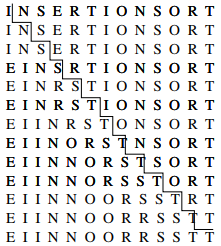
\includegraphics[scale=0.6]{./insertion_sort.png}
  \label{fig:demo-diagram}
  \caption{Animation of insertion sort in action (time flows down)}
\end{figure}


\begin{verbatim}
insertion_sort(item s[], int n)
{
    int i,j; /* counters */

    for (i=1; i<n; i++) {
        j=i;
        while ((j>0) && (s[j] < s[j-1])) {
            swap(&s[j], &s[j-1]);
            j = j-1;
        }
    }
}
\end{verbatim}

\noindent\rule{\textwidth}{0.4pt}


\begin{figure}[H]
  \centering
     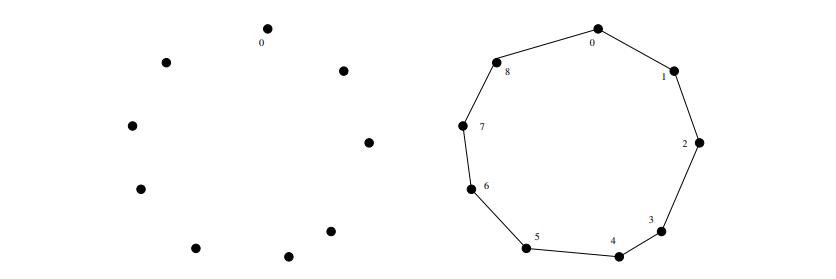
\includegraphics[scale=0.6]{./nearest_neighbor.png}
  \label{fig:demo-diagram2}
  \caption{A good instance for the nearest neighbor heuristic}
\end{figure}




\subsection{Robot Tour Optimization}
aaa
\subsection{Selecting the Right Jobs}
bbb

\subsubsection{test, delete this}
\subsection{Reasoning about Correctness}

\subsubsection{Expressing Algorithms}
\subsection{Modeling The Problem}

\subsubsection{Combinatorial Objects}

\subsubsection{Recursive Objects}
\subsection{About the War Stories}


\subsection{War Story: Psychic Modeling}

\section{Algorithm Analysis}
Our two most important tools are 
\begin{enumerate}
	\item
	  \emph{The RAM model of
			computation}
	\item
	  \emph{The asymptotic analysis of worst-case complexity}
\end{enumerate}

\subsection{The RAM Model of Computation}

\subsubsection{Best, Worst, and Average-Case Complexity}

\subsection{The Big Oh Notation}
\subsection{Growth Rates and Dominance Relations}

\begin{figure}[H]
  \centering
     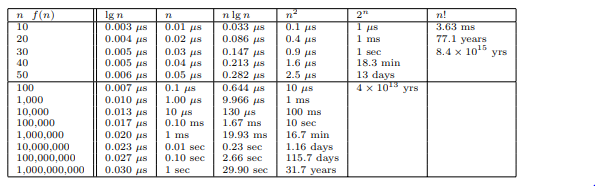
\includegraphics[scale=1.0]{./2_4.png}
  \label{fig:demo-diagram2-4}
  \caption{ Growth rates of common functions measured in nanoseconds}
\end{figure}


\subsubsection{Dominance Relations}

\noindent\fbox{\parbox{\textwidth}{%
\emph{Take-Home Lesson: }Although esoteric functions arise in advanced algorithm
analysis, a small variety of time complexities suffice and account for most
algorithms that are widely used in practice.
}%
}



\subsection{Working with the Big Oh}

\subsubsection{Adding Functions}

$$O(f(n)) + O(g(n)) \longrightarrow O(max(f(n),g(n))$$

$$\Omega(f(n)) + \Omega(g(n)) \longrightarrow \Omega(max(f(n),g(n))$$


$$\Theta(f(n)) + \Theta(g(n)) \longrightarrow \Theta(max(f(n),g(n))$$

\subsubsection{Multiplying Functions}

$$O(c*f(n))) \longrightarrow O(f(n))$$

$$\Omega(c*f(n))) \longrightarrow \Omega(f(n))$$


$$\Theta(c*f(n))) \longrightarrow \Theta(f(n))$$

\noindent\rule{\textwidth}{0.4pt}

$$O(f(n)) * O(g(n)) \longrightarrow O(f(n) * g(n))$$

$$\Omega(f(n)) * \Omega(g(n)) \longrightarrow \Omega(f(n) * g(n))$$

$$\Theta(f(n)) * \Theta(g(n)) \longrightarrow \Theta(f(n) * g(n))$$

\noindent\rule{\textwidth}{0.4pt}

\textbf{Stop and Think: Hip to the SquaresTransitive Experience} \\

\emph{Show that Big Oh relationships are transitive. That is, if $f(n) = O(g(n))$ and $g(n) = O(h(n))$, then $f(n) = O(h(n))$}
\subsection{Reasoning About Efficiency}

\subsubsection{Selection Sort}

\subsubsection{Insertion Sort}

\subsubsection{String Pattern Matching}

\subsubsection{Matrix Multiplication}
\subsection{Logarithms and Their Applications}
$$b^{x} = y \leftrightarrow x = log_{b}y$$
$$b^{log_{b}y} = y$$

\subsubsection{Logarithms and Binary Search}

\begin{figure}[H]
  \centering
     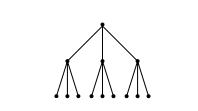
\includegraphics[scale=0.9]{./2_7.png}
  \label{fig:demo-diagram2-4}
  \caption{ A height \emph{h} tree with \emph{d} children per node as \emph{$d^{h}$} leaves. Here $h=2$ and $d=3$}
\end{figure}


\subsubsection{Logarithms Trees}

\subsubsection{Logarithms and Bits}

\subsubsection{Logarithms and Multiplication}

\begin{align*}
	&log_{a}(xy) = log_{a}(x) + log_a(y) \\
	&log_{a} n^{b} = b \cdot log_{a} n \\
	&a^{b} = e^{(ln(a^{b}))} = e^{(b(ln(a)))}
\end{align*}

\subsubsection{Fast Exponentiation}

\subsubsection{Logarithms and Summations}

\emph{Harmonic Numbers}: 
$$H(n) = \sum_{i=1}^{n} \frac{1}{i} \sim ln(n)$$

\subsubsection{Logarithms and Criminal Justice}


\begin{figure}[H]
  \centering
     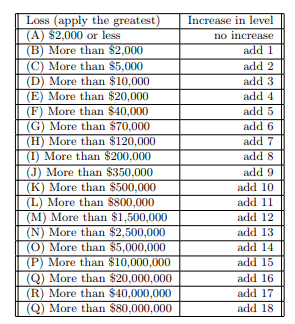
\includegraphics[scale=0.9]{./2_8.png}
  \label{fig:demo-diagram2-8}
  \caption{The Federal Sentencing Guidelines for fraud}
\end{figure}

\noindent\fbox{\parbox{\textwidth}{%
\emph{Take-Home Lesson: } Logarithms arise whenever things are repeatedly halved or doubled
}%
}

\subsection{Properties of Logarithms}

$$log_{a}b = \frac{log_{c}b}{log_{c}a}$$

\textbf{Stop and Think: Importnce of an Even Split} \\

\emph{How many queries does binary search take on the million-name Manhattan phone boo if each split was 1/3 to 2/3 instead of 1/2 to 1/2?}
\subsection{War Story: Mystery of the Pyramids}
\subsection{Advanced Aanalysis (*)}

\subsection{Esoteric Functions}

\subsection{Limits and Dominance Relations}

\noindent\fbox{\parbox{\textwidth}{%
\emph{Take-Home Lesson: } By interleaving the functions here with those of Section 2.3.1 we see where everything fits into the dominnce pecking order:
$$n! \gg c^{n} \gg n^{3} \gg n^{2} \gg n^{1 + \epsilon} \gg n\cdot log(n) \gg n \gg \sqrt{n}$$
$$ \gg log^{2}n \gg log(n) \gg \frac{log(n)}{log(log(n))} \gg log(log(n)) \gg \alpha (n) \gg 1$$
}%
}

\section{Data Structures}
3 Fundamental abstract data types

\begin{itemize}
	\item \emph{Containers}
	\item \emph{Dictionaries}
	\item \emph{Lists}
\end{itemize}
\subsection{Contigous vs. Linked Data Structures}

\begin{itemize}
	\item 
	  \emph{Continuously allocated structures (arrays)}
	\item 
	  \emph{Linked data structures (pointers, lists, trees...)}
\end{itemize}

\subsubsection{Arrays}
$$M=\sum_{i=1}^{lg(n)} i*\frac{n}{2^{i}} = n*\sum_{i=1}^{lg(n)}\frac{i}{2^{i}} \leq n*\sum_{i=1}^{\infty}\frac{i}{2^{i}} = 2n$$

\subsubsection{Pointers and Linked Structures}

figure here*** (Linked Lst example showing data and pointer fields)

\begin{verbatim}
  typedef struct list {
    item_type item;          /*data item*/
    struct list *next;       /*point to successor*/
  } list;
\end{verbatim}

\textbf{ \emph{Searching a List} }\\

\begin{verbatim}
  list *search_list(list *1, item_type x)
  {
    if(1 == NULL) return(NULL);

    if(1->item == x)
      return(1);
    else
      return(search_list(1->next, x) );
  }
\end{verbatim}

\textbf{ \emph{Insertion into a List} }\\

\begin{verbatim}
  void insert_list(list **1, item_type x) 
  {
      list *p                  /* temporary pointer*/

      p = malloc(sizeof(list));
      p->item = x;
      p->next = *1;
      *1 = p;
  }
\end{verbatim}

\textbf{ \emph{Deletion From a List} }\\

\begin{verbatim}
  list *predecessor_list(list *1, item_type x)
  {
      if((1 == NULL) || (1->next == NULL)) {
          printf("Error: predecessor sought on null list.\n");
          return(NULL);
      }

      if((1->next)->item == x)
          return(1);
      else
          return(predecessor_list(1->next, x));
  }

  delete_list(list **1, item_type x)
  {
      list *p;                      /*item pointer*/
      list *pred                    /*predecessor pointer*/
      list *search_list(), *predecessor_list();

      p = search_list(*1,x);
      if(p != NULL) {
          pred = predecessor_list(*1, x);
          if(pred == NULL)          /*splice out list*/
              *1 = p->next;
          else
              pred->next = p->next;
          free(p);                  /*free memory used by node*/
      }
  }
\end{verbatim}

\subsubsection{Comparison}

\noindent\fbox{\parbox{\textwidth}{%
\emph{Take-Home Lesson: }Dynamic memory allocation provides us with flexibility on how and where we use our limited storage resources.
}%
}
\subsection{Stacks and Queues}

\begin{itemize}
	\item \emph{\textbf{Stacks:} LIFO}
	\item \emph{\textbf{Queues:} FIFO}
\end{itemize}
\subsection{Dictionaries}

\textbf{\emph{Primary Operations:}}

\begin{enumerate}
	\item Search
	\item Insert
	\item Delete
\end{enumerate}

\textbf{Stop and Think: Comparing Dictionary Implementations (I)} \\

\emph{Problem: What are the asymptotic worst-case running times for each of the seven fundamental dictionary operations (search, delete, successor, predecessor, minimum, maximum) when the data structure is implemented as:}\\

\begin{enumerate}
	\item \emph{An unsorted array}
	\item \emph{A sorted Array}
\end{enumerate}

\noindent\fbox{\parbox{\textwidth}{%
\emph{Take-Home Lesson: }Data structure design must balance all the different operations it supports. The fastest data structure to support both operations A and B may well not be the fastest structure to supprt either operation A or B.
}%
}

\textbf{Stop and Think: Comparing Dictionary Implementations (II)} \\

\emph{Problem: What are the asymptotic worst-case running times for each of the seven fundamental dictionary operations (search, delete, successor, predecessor, minimum, maximum) when the data structure is implemented as:}\\

\begin{enumerate}
	\item \emph{A singly-linked unsorted list}
	\item \emph{A doubly-linked unsorted list}
	\item \emph{A singly-linked sorted list}
	\item \emph{A doubly-linked sorted list}
\end{enumerate}
\subsection{Binary Search Trees}

For any binary tree on n nodes and any set of n keys, there is exactly one labeling that makes it a binary search tree \\

\subsubsection{Implementing Binary Search Trees}

\begin{verbatim}
    typedef struct tree {
        item_type item;        /*data item*/
        struct tree *parent    /*pointer to parent*/
        struct tree *left      /*pointer to left child*/
        struct tree *right     /*pointer to right child*/
    } tree;
\end{verbatim}

Basic binary search tree operations:
\begin{itemize}
	\item \emph{search}
	\item \emph{traversal}
	\item \emph{insertion}
	\item \emph{deletion}
\end{itemize}

\textbf{ \emph{Searching in a Tree} }\\

\begin{verbatim}
    tree *search_tree(tree *1, item_type x)
    {
        if(1 == NULL) return(NULL);

        if(1->item == x) return(1);

        if(x < 1->item)
            return(search_tree(1->left, x));
        else
            return(search_tree(1->right, x));
    }
\end{verbatim}

\textbf{ \emph{Finding Minimum and Maximum Elements in a Tree} }\\

\begin{verbatim}
    tree *find_minimum(tree *t)
    {
        tree *min;         /*pointer to minimum*/

        if(t == NULL) return(NULL);

        min = t;
        while(min->left !=NULL)
            min = min->left;
        return(min)
    }
\end{verbatim}

\textbf{ \emph{Traversal in a Tree} }\\

\begin{verbatim}
    void traverse_tree(tree *1)
    {
        if(1 != NULL) {
            traverse_tree(1->left);
            process_item(1->item);
            traverse_tree(1->right);
        }
    }
\end{verbatim}

\textbf{ \emph{Insertion in a Tree} }\\

\begin{verbatim}
    insert_tree(tree **1, item_type x, tree *parent)
    {
        tree *p;                          /*temporary pointer*/

        if(*1 == NULL) {
            p = malloc(sizeof(tree));     /*allocate new node*/
            p->item = x;
            p->left = p->right = NULL;
            p->parent = parent;
            *1 = p;                       /*link into parents record*/
            return;
        }

        if(x < (*1)->item)
            insert_tree(&((*1)->left), x, *1);
        else
            insert_tree(&((*1)->right), x, *1);
    }
\end{verbatim}

\textbf{ \emph{Deletion from a Tree} }\\

figure here*** (Deleting tree nodes with 0, 1 and 2 children)\\

\subsubsection{How Good Are Binary Search Trees?}

What if items are inserted in order? Trees should be balanced. \\


\subsubsection{Balanced Search Trees}

\noindent\fbox{\parbox{\textwidth}{%
\emph{Take-Home Lesson: }Picking the wrong data structure for the job can be disastrous in terms of performance. Identifying the very best data structure is usually not as critical, because there can be several choices that perform similarly.
}%
}

\textbf{Stop and Think: Exploiting Balanced Search Trees} \\

\emph{Problem: You are given the task of reading n numbers and then printing them out in sorted order. Suppose you have access to a balanced dictionary data structure, which supports the operations search, insert, delete, minimum, maximum, successor and predecesor each in O(log(n)) time}\\

\begin{enumerate}
	\item \emph{How can you sort in O(nlog(n)) time using only insert and in-order traversal?}
	\item \emph{How can you sort in O(nlog(n)) time using only minimum, seccessor, and insert?}
	\item \emph{How can you sort in O(nlog(n)) time using only minimum, insert, delete, and search?}
\end{enumerate}







% -- Bibliography (APA)
% \bibliography{references}

\end{document}